\subsection{Converting a balanced product to a feature}
\label{subsec:contour-conversion}

Lemma~\ref{lem:balanced-product} supplies a product of at most four windowed
Fourier sums with a substantial discrepancy and small total frequency.
We now express that product as an integral of features. The contour will
place their outer parameters in the sector required by
Proposition~\ref{prop:multiscale}; the remaining issue will be to control
the damping factors on their inner gaps.

Fix a product supplied by Lemma~\ref{lem:balanced-product}, and let
$1\le m\le4$ be its number of factors. Expand each factor in the tuples
defining $f$. An \emph{interleaving} specifies the ordering, including all
ties, of the $mk$ labeled positions in these tuples. There are at most
$(mk)^{mk}=\exp(O(k\log(2k)))$ interleavings: assigning to each labeled
position its rank among the distinct positions gives such a bound.
Only interleavings consistent with strict increase inside each old tuple
are retained. Fix one interleaving, and relabel its copies so that their
endpoints satisfy $j_1\le\cdots\le j_m$. Equal endpoints may be ordered
arbitrarily. After absorbing conjugation into the signs of the
frequencies, their window weight is
\begin{equation}
 \prod_{r=1}^m W(j_r-d)\exp\bigl(\ii t_r(j_r-d)\bigr),
 \qquad |t_r|\le C_3S,\qquad
 \left|\sum_{r=1}^m t_r\right|\le b.
 \label{eq:endpoint-window}
\end{equation}
Conjugation also conjugates the old inner-gap parameters, leaving their
dampings unchanged.

\paragraph{A Gaussian contour with controlled total frequency.}
Recall that $\sigma=K\sqrt E/S'$ and $b=\beta S'$. For every real $l$,
\begin{equation}
 W(l)=\frac{\sigma}{\ii\sqrt{2\pi}}
       \int_{-\ii\infty}^{\ii\infty}
       \exp(\sigma^2v^2/2+vl)\,dv.
 \label{eq:gaussian-contour}
\end{equation}
Indeed, writing $v=\ii u$ gives the Gaussian Fourier transform. Its value
at $l=0$ is one, and integration by parts shows that its derivative in
$l$ is $-l/\sigma^2$ times itself, proving the formula.

Set $\rho=1/2.002$. For $u=(u_1,\ldots,u_m)\in\RR^m$, define
\begin{equation}
 \Omega=\sum_{r=1}^m(u_r+t_r),\qquad
 v_r=b+\ii u_r\quad(r<m),\qquad
 v_m=-mb-\rho|\Omega|+\ii u_m.
 \label{eq:bent-contour}
\end{equation}
These real parts have partial sums $rb$ for $r<m$ and total sum
$-b-\rho|\Omega|$. When the endpoint exponent is centered at $j_m$,
the total sum gives the real part of its outer coefficient, while the
negatives of the partial sums give the real parts of the coefficients
on consecutive endpoint gaps. The contour is
therefore designed to give outer decay $b+\rho|\Omega|$ and positive
inner dampings $rb$; we verify the exact rewriting below.

For each fixed tuple of positions, first shift the first $m-1$ contours
in \eqref{eq:gaussian-contour} to their fixed vertical lines
$\re v_r=b$, leaving the last contour on the imaginary axis.
The connecting horizontal integrals vanish by Gaussian decay.
Next fix $(u_1,\ldots,u_{m-1})$ and deform the last contour to the
piecewise linear graph in \eqref{eq:bent-contour}. Its slopes have
absolute value $\rho<1$. Along horizontal segments joining its
truncations to the imaginary axis at height $\pm T$, the Gaussian
exponent has real part at most $-cT^2+O(T)$ for some $c>0$.
The factor $\exp(v_m(j_m-d))$ contributes only a linear term in $T$,
so these connecting integrals also vanish. The integrands are entire,
and hence no residues occur. This proves the identities as iterated
integrals; absolute joint convergence will follow from the next bound.

Let $\nu$ be the resulting complex measure on $\RR^m$ after the factors
depending on positions have been removed. More explicitly, outside the
measure-zero set $\Omega=0$,
\begin{equation}
 d\nu(u)=
 \left(\frac{\sigma}{\sqrt{2\pi}}\right)^m
 \exp\left(\frac{\sigma^2}{2}\sum_{r=1}^m v_r^2\right)
 \bigl(1+\ii\rho\operatorname{sgn}\Omega\bigr)\,du.
 \label{eq:contour-measure}
\end{equation}
The last factor is the differential of the bent contour divided by
$\ii\,du_m$. We next obtain estimates uniform over the frequencies in
\eqref{eq:endpoint-window}. These estimates also establish absolute
convergence of the joint integrals.

Put $\delta_0=1-4\rho^2>0$ and $c_1=\delta_0/2$. Since $m\le4$ and
$|\sum t_r|\le b$, Young's inequality gives an absolute $C_4$ such that
\begin{align}
 \sum_{r=1}^m(\re v_r)^2
 &=(m-1)b^2+(mb+\rho|\Omega|)^2 \notag\\
 &\le 3b^2+
       \left(2\rho\sqrt{\sum_r u_r^2}+(4+\rho)b\right)^2 \notag\\
 &\le (1-c_1)\sum_r u_r^2+C_4b^2.
 \label{eq:contour-quadratic}
\end{align}
The strict inequality $4\rho^2<1$ is essential here: summing at most
four imaginary coordinates can multiply their squared norm by four,
and the sector constant $2.002$ leaves a positive Gaussian decay margin.
For example,
$C_4=3+(4+\rho)^2(1+8\rho^2/\delta_0)$ suffices.
Together with \eqref{eq:contour-measure}, this proves
\[
 |d\nu(u)|\le C\sigma^m
 \exp\left(\frac{C_4\sigma^2b^2}{2}
           -\frac{c_1\sigma^2}{2}\sum_r u_r^2\right)du.
\]
For any fixed tuple of positions, the absolute value of its remaining
exponential factor is at most $\exp(C_n(1+\sum_r|u_r|))$ for a finite
constant $C_n$. This factor is integrable against the Gaussian bound.
Thus the iterated deformation also gives a jointly absolutely
convergent integral, and finite tuple sums can be interchanged with it.

Write $\mathcal U=\{u:\max_r|u_r|\le S'/16\}$. Integrating the last
bound, and splitting its negative quadratic term into two equal parts
on $\mathcal U^c$, gives absolute constants $C,C'$ with
\begin{align*}
 \|\nu\|_{\mathrm{abs}}
   &\le C\exp(C_4K^2\beta^2E/2),\\
 \int_{\mathcal U^c}|d\nu|
   &\le C'\exp\left[
      \left(\frac{C_4K^2\beta^2}{2}
                 -\frac{c_1K^2}{1024}\right)E\right].
\end{align*}
Here $\|\nu\|_{\mathrm{abs}}$ denotes total variation; the powers
$\sigma^m$ cancel under Gaussian rescaling. Choose $K$ large enough that
$c_1K^2/1024\ge30$, then choose $\beta\le1/4$ small enough that
$C_4K^2\beta^2/2\le0.001$. Increasing $C_0$ to absorb the fixed
prefactors yields
\begin{equation}
 \|\nu\|_{\mathrm{abs}}\le e^{0.005E},\qquad
 \int_{\mathcal U^c}|d\nu|\le e^{-20E}.
 \label{eq:contour-mass}
\end{equation}
This choice is consistent with the order of constants specified earlier:
$K$ is fixed first, $\beta$ second, and $\eta_0$ may then be reduced to
meet the window estimate. Only afterward is $C_0$ enlarged.

\paragraph{Outer parameters and endpoint gaps.}
For $c_r=v_r+\ii t_r$, telescoping the endpoint differences gives
\begin{equation}
 \sum_{r=1}^m c_r(j_r-d)
 =\left(\sum_{r=1}^m c_r\right)(j_m-d)
  -\sum_{r=1}^{m-1}
    \left(\sum_{l=1}^r c_l\right)(j_{r+1}-j_r).
 \label{eq:endpoint-telescoping}
\end{equation}
Consequently, the largest endpoint has coefficient
$-s'+\ii\Omega$, where
\begin{equation}
 s'=b+\rho|\Omega|.
 \label{eq:new-outer-decay}
\end{equation}
The link from $j_r$ to $j_{r+1}$ receives the parameter
\begin{equation}
 \exp\left(-rb-\ii\sum_{l=1}^r(u_l+t_l)\right),
 \qquad 1\le r<m.
 \label{eq:endpoint-link}
\end{equation}
Thus every added damping is at least $b$, for every $u$.
On $\mathcal U$,
\[
 |\Omega|\le(\beta+1/4)S',\qquad
 \beta S'\le s'\le
   \bigl[\beta+\rho(\beta+1/4)\bigr]S'\le S',
 \qquad |\Omega|\le2.002s'.
\]
The angle in \eqref{eq:endpoint-link} has absolute value at most
$3(C_3S+S'/16)\le C_1S$ for a fixed absolute $C_1$.
The outer parameters therefore satisfy the parameter inequalities in
\eqref{eq:multiscale-output}, and the endpoint links satisfy
\eqref{eq:added-parameters}. The choice of $C_1$ uses only $C_3$ and
$S'\le S$ and imposes no further condition on $K$ or $\beta$.

\subsection{Interleavings and the cost of the inner gaps}
\label{subsec:interleavings}

We have obtained outer weights at the required scale. To finish, we must
show that each interleaving has exactly the form of a feature, with
controlled coefficient sum. One old inner edge can cross several gaps
of the merged tuple, so charging its damping cost at every crossing
would overcount it. A distinct-edge assignment will prevent this loss.

For our fixed interleaving, write its distinct positions as
$i_1<\cdots<i_v$, where $1\le v\le mk$. Form a multigraph on these
vertices: include the inner edges of each old tuple and the links
between consecutive endpoints in \eqref{eq:endpoint-link}. Its edges
carry their corresponding exponential parameters. It is connected,
because each old tuple is a path to its endpoint, and the endpoint
links join those paths. Delete loops coming from equal endpoints;
their weights are one.

For each merged gap $i_{a+1}-i_a$, multiply the parameters of all edges
crossing it. Each edge length is the sum of the merged gaps it crosses,
so these new parameters reproduce the original weight exactly.
Every merged gap is crossed by some edge, by connectivity, and hence
its damping is positive. Within a single old tuple, the inner-edge
intervals have disjoint interiors. The same holds for the consecutive
endpoint links. It follows that each new parameter uses at most one
old parameter from each copy and at most one added endpoint parameter.
This is precisely the factor-count assertion in
Proposition~\ref{prop:multiscale}.

Ties merge repeated bit variables by the Boolean identity $X_i^r=X_i$
for $r\ge1$. Once the interleaving is fixed, choosing arbitrary strictly
increasing values for its $v$ distinct positions specifies exactly one
assignment to its labeled tuples. Thus no further restriction remains
on the new tuple. Its largest position is $i_v=j_m$. Summing all these
assignments gives an order-$v$ feature, denoted $f^{\mathcal I,u}$,
with outer weight $\exp((-s'+\ii\Omega)(i_v-d))$.

The following elementary fact controls its height.

\begin{lemma}[Assigning distinct edges to consecutive gaps]
\label{lem:edge-gap-assignment}
Let a connected multigraph have ordered vertices $i_1<\cdots<i_v$.
There is an assignment of a distinct edge to each gap
$(i_a,i_{a+1})$ such that its assigned edge crosses that gap.
\end{lemma}

\begin{proof}
There is nothing to prove for $v=1$. Otherwise retain a spanning tree
and orient each of its edges from its smaller to its larger endpoint.
Let $M$ be the $(v-1)\times(v-1)$ matrix whose $(e,a)$ entry is one if
tree edge $e$ crosses gap $a$, and zero otherwise. This matrix is
invertible. To see this, for an arbitrary vector $g$ in its kernel set
$y_1=0$ and $y_{a+1}=y_a+g_a$. The equation $Mg=0$ says that $y$ has
equal values at the endpoints of every tree edge. Connectivity makes
all its values zero, so $g=0$. A nonzero term in the determinant
expansion of $M$ pairs its rows and columns through entries equal to
one. That pairing is the required assignment.
\end{proof}

Figure~\ref{fig:edge-gap-assignment} shows why distinctness matters.
Although one edge may contribute to several new parameters, it need
pay for only one of their upper bounds.

\begin{figure}[htbp]
\centering
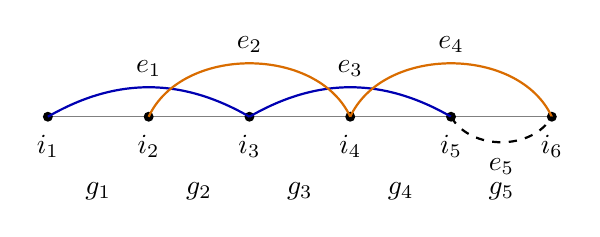
\begin{tikzpicture}[x=1.28cm,y=0.9cm,>=stealth,
  olda/.style={draw=blue!70!black,thick},
  oldb/.style={draw=orange!85!black,thick},
  added/.style={draw=black,thick,dashed}]
  \draw[gray] (0,0)--(5,0);
  \foreach \a in {1,...,6} {
    \fill (\a-1,0) circle (1.8pt);
    \node[below=3pt] at (\a-1,0) {$i_{\a}$};
  }
  \draw[olda] (0,0) to[bend left=30] node[above,pos=.5] {$e_1$} (2,0);
  \draw[olda] (2,0) to[bend left=30] node[above,pos=.5] {$e_3$} (4,0);
  \draw[oldb] (1,0) to[bend left=65] node[above,pos=.5] {$e_2$} (3,0);
  \draw[oldb] (3,0) to[bend left=65] node[above,pos=.5] {$e_4$} (5,0);
  \draw[added] (4,0) to[bend right=60] node[below=2pt,pos=.5] {$e_5$} (5,0);
  \foreach \a in {1,...,5} {
    \node at (\a-.5,-1.05) {$g_{\a}$};
  }
\end{tikzpicture}
\caption{A schematic interleaving of the two old tuples
$(i_1,i_3,i_5)$ and $(i_2,i_4,i_6)$, joined by the dashed endpoint link
$e_5$. Here $g_a$ denotes the gap $(i_a,i_{a+1})$.
The assignment $g_a\mapsto e_a$ for $1\le a\le5$ uses a distinct
crossing edge for every gap. For example,
$e_1$ crosses both $g_1$ and $g_2$, but it is charged only to $g_1$;
$e_2$ supplies the bound for $g_2$.}
\label{fig:edge-gap-assignment}
\end{figure}

Give each edge occurrence $e$ its damping $a_e>0$. The damping of a
merged gap is the sum of the $a_e$ over all edges crossing it, and is
therefore at least that of its assigned edge. Since $1+1/a$ decreases
with $a$, Lemma~\ref{lem:edge-gap-assignment} implies
\begin{align}
 H_{f^{\mathcal I,u}}
 &\le\prod_{e\text{ assigned}}(1+1/a_e)
 \le\prod_{e\text{ present}}(1+1/a_e) \notag\\
 &\le H_f^m(1+1/b)^{m-1}
 \le H_f^4(1+1/b)^3.
 \label{eq:interleaving-height}
\end{align}
The second inequality uses that all factors are at least one; the
endpoint-link dampings are $rb\ge b$. This argument includes all
overlaps between old tuples and also the case of a single distinct
position. In that case the height is the empty product one.

\paragraph{Completing the multiscale estimate.}
Apply $\Delta$ to the expanded product and use the integral
representation for each interleaving. With $\nu_{\mathcal I}$ denoting
the corresponding measure, we have the exact identity
\begin{equation}
 \Delta[\text{product}]
 =\sum_{\mathcal I}\int_{\RR^m}
   \mathcal S_{f^{\mathcal I,u}}(s',\Omega)\,d\nu_{\mathcal I}(u).
 \label{eq:product-feature-integral}
\end{equation}
All estimates above are uniform over the interleavings. The integrands
have a uniform bound even outside $\mathcal U$. Indeed, for each fixed
endpoint $j$, the coefficients of $f_j^{\mathcal I,u}$ have absolute
sum at most the height in \eqref{eq:interleaving-height}. The terms with
endpoint $j<d$ vanish under $\Delta$ by prefix agreement.
Using $s'\ge b$ gives
\begin{equation}
 \left|\mathcal S_{f^{\mathcal I,u}}(s',\Omega)\right|
 \le 2H_f^4(1+1/b)^3\sum_{l\ge0}e^{-bl}
 \le 2H_f^4(1+1/b)^4.
 \label{eq:contour-uniform-signal}
\end{equation}
In particular no exponential factor from negative distances occurs
in the tail estimate.

Let $N_{\mathrm{int}}$ be the number of interleavings and put
$V=2H_f^4(1+1/b)^4$. Hypothesis~\eqref{eq:multiscale-cost}, with a
sufficiently large absolute $C_0$, ensures
\[
 E\ge100,\qquad \log N_{\mathrm{int}}\le0.01E,
 \qquad \log V\le0.01E.
\]
Here $\log(1+1/b)$ is bounded by an absolute constant plus
$\log(1/S')$, because $b=\beta S'$, $S'\le1$, and $\beta$ has already
been fixed. If every signal in \eqref{eq:product-feature-integral}
with $u\in\mathcal U$ had magnitude below $e^{-7.98E}$, then
\eqref{eq:contour-mass} and \eqref{eq:contour-uniform-signal} would give
\[
 |\Delta[\text{product}]|
 \le N_{\mathrm{int}}
       \left(e^{(0.005-7.98)E}+Ve^{-20E}\right)
 \le e^{-7.965E}+e^{-19.98E}
 <e^{-7.94E}.
\]
This contradicts Lemma~\ref{lem:balanced-product}. Some interleaving
and some $u\in\mathcal U$ therefore give a feature with signal at least
$e^{-7.98E}$. Its order is at most $mk\le4k$;
\eqref{eq:new-outer-decay} and the bounds on $\mathcal U$ give the
required outer parameters; \eqref{eq:interleaving-height} gives
\eqref{eq:multiscale-height}; and the crossing description gives the
claimed parameter factors and \eqref{eq:added-parameters}.
This completes the proof of Proposition~\ref{prop:multiscale}.
